\begin{frame}
	\frametitle{Les échanges \textit{off chain}}
	\begin{itemize}
		\item Ils s'effectuent en dehors de la blockchain principale $\Rightarrow$ \textit{layer 2}.
		\item Permettent d'avoir un compromis avec la blockchain principale.
		\item Les chaines ne sont pas vouées à être fusionné avec la blockchain mère.
	\end{itemize}
\end{frame}

\begin{frame}
	\frametitle{Les échanges \textit{off chain}: Visualisation}
	\begin{figure}[h!]
		\centering
		\stackunder{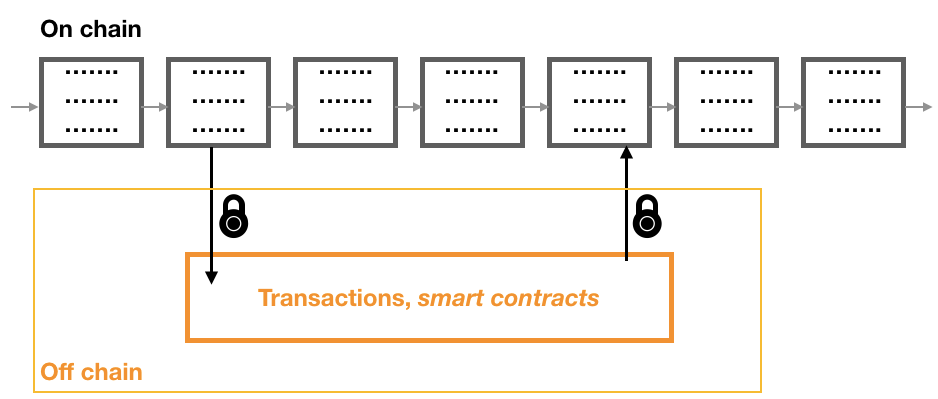
\includegraphics[scale=0.37]{decentralisation/offchain.png}}
		{\scriptsize Source: \url{www.cryptoencyclopedie.com}}
		\label{fig:offchain}
	\end{figure}
\end{frame}


\begin{frame}
	\frametitle{Exemple d'échange \textit{off chain}: Le réseau Lightning}
	\begin{itemize}
		\item Couche secondaire de la blockchain Bitcoin. \newline
		\item Permet de faire des transactions en dehors de la blockchain principale $\Rightarrow$ off-chain. \newline
		\item Échanges par canaux bidirectionnels.
	\end{itemize}
\end{frame}


\begin{frame}
	\frametitle{Le réseau Lightning (Lightning Network) - Fonctionnement }
	\begin{figure}[h!]
		\stackunder{
			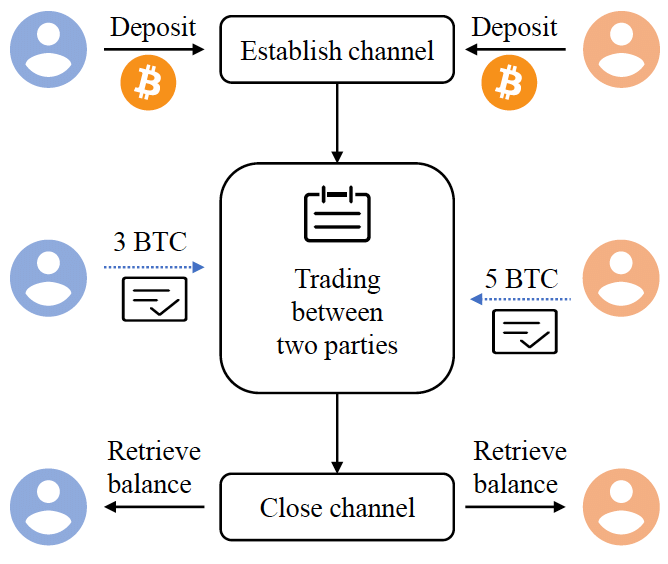
\includegraphics[scale = 0.3 ]{decentralisation/Procedures-of-Lightning-network.png}  }
		{\scriptsize Source: \url{https://issam.ma/jekyll/update/2022/03/01/bitcoin-must-die-5.html}}

		\caption{Le réseau Lightning par rapport à la \textit{blockchain} Bitcoin principale}

	\end{figure}

\end{frame}

\begin{frame}
	\frametitle{Le réseau Lightning (Lightning Network) - Avantages}
	\begin{itemize}
		\item Aucune limite sur le nombre de transactions par seconde sur le réseau.
		      \newline
		\item Des transactions instantanées. Plus d’attente de confirmation par les mineurs.
		      \newline
		\item Des frais de transaction extrêmement faibles ouvrant la voie aux micro-transactions.
	\end{itemize}
\end{frame}

\begin{frame}
	\frametitle{Implémentation du MIT}
	Implémentaion des swaps atomiques sur le réseau Lightning par le MIT. Les objectifs sont :
	\newline
	\begin{itemize}
		\item Permettre d'utiliser le réseau Lightning sur des blockchains différentes.
		\item Permettre des échanges sur des blockchains non monétaires.
		\item Proposer une interface pour des échanges cross-chain.
	\end{itemize}

\end{frame}


\begin{frame}
	\frametitle{Implémentation du MIT - Limitations}


	\begin{itemize}
		\item Il n'y a pas de support de channel hopping malgré l'utilisation du réseau Lightning.
		      \begin{itemize}
			      \item Cela implique des problème de mise à l'échelle.
		      \end{itemize}
		\item Il n'y a pas de vérification sur les valeurs inscrites sur les chaines non monétaires.
		\begin{itemize}
			\item Risque accru de perte financière.
		\end{itemize}
	\end{itemize}
\end{frame}
